\newpage
\section{Latex-Details}

\subsection{Verwendete Software, Editor und Zusatzpakete}
\subsubsection{Windows 8+}
\begin{itemize}
\item MikTex: 2.9, 32-bit
\item Biblatex: 3.5, Zusatz: Biber.exe
\item Editor: TexStudio (kann ich empfehlen), Notepad++
\end{itemize}

\subsubsection{Mac OSX und iOS}
\begin{itemize}
\item MacTeX: \url{https://tug.org/mactex}
\item Editor: TexPad \url{https://www.texpadapp.com}

\subsubsection{Online}
Overleaf ist eine Online-Anwendung mit der Ihr direkt im Browser an eurer Thesis schreiben könnt. Bis 1GB Größe und maximal 60 Einzeldateien könnt ihr Overleaf kostenlos nutzen: \url{https://www.overleaf.com/}


\subsection{Dokumentenklasse}
Eigentlich hatte Prof. Finke empfohlen die Dokumentklassen \enquote{Book} oder \enquote{Report} für die Erstellung der Bachelor-Thesis zu verwenden, da diese über weitere Gliederungsebenen verfügen. Ich verwende dennoch eine leicht modifizierte Komaskript-Klasse \enquote{scrartcl}, mit der Erweiterung um eine Ebene. Siehe (skripte/weitereEbene.tex). Das Skript stammt irgendwo aus den Netz und übersteigt meine \LaTeX{}-Fähigkeiten. Dadurch kann ich über eine weitere Ebene in der Arbeit verfügen, ohne mich mit der Modifikation von Kapitel-Seiten rumschlagen~\footcite[Vgl. ][Seite 5]{Tanenbaum.2003} zu müssen. Diese Quelle ist nur zur Demonstration und hat keinen inhaltlichen Bezug hierzu. Es werden übrigens nur die Quellen im Literaturverzeichnis angezeigt, die auch referenziert sind.


\subsection{Grafiken}
Das Paket \textbackslash usepackage\{float\} ermöglicht es die Grafiken und Tabellen an der Stelle im Text zu positionieren, wo diese im Quelltext stehen (Option H). Ansonsten würde \LaTeX{} diese dort unterbringen, wo es typographisch sinnvoll wäre - das wollen wir ja nicht ;-).

Die Breite der Grafiken am Besten relativ zum Text angeben.

\subsection{Quellcode}
Quellcode kann auf unterschiedliche Arten eingebaut werden.
Zum einen kann es hier durch direktives Einbinden in der Kapitel-Datei geschehen.
\begin{lstlisting}
% Hier wird aufgezeigt, wie man eine Grafik einbindet, es wird also in der PDF angezeigt,
% da es in einem Quellcode-Listing steht.
% Auch wenn es hier faelschlicherweise als LaTeX-Befehl angezeigt wird.
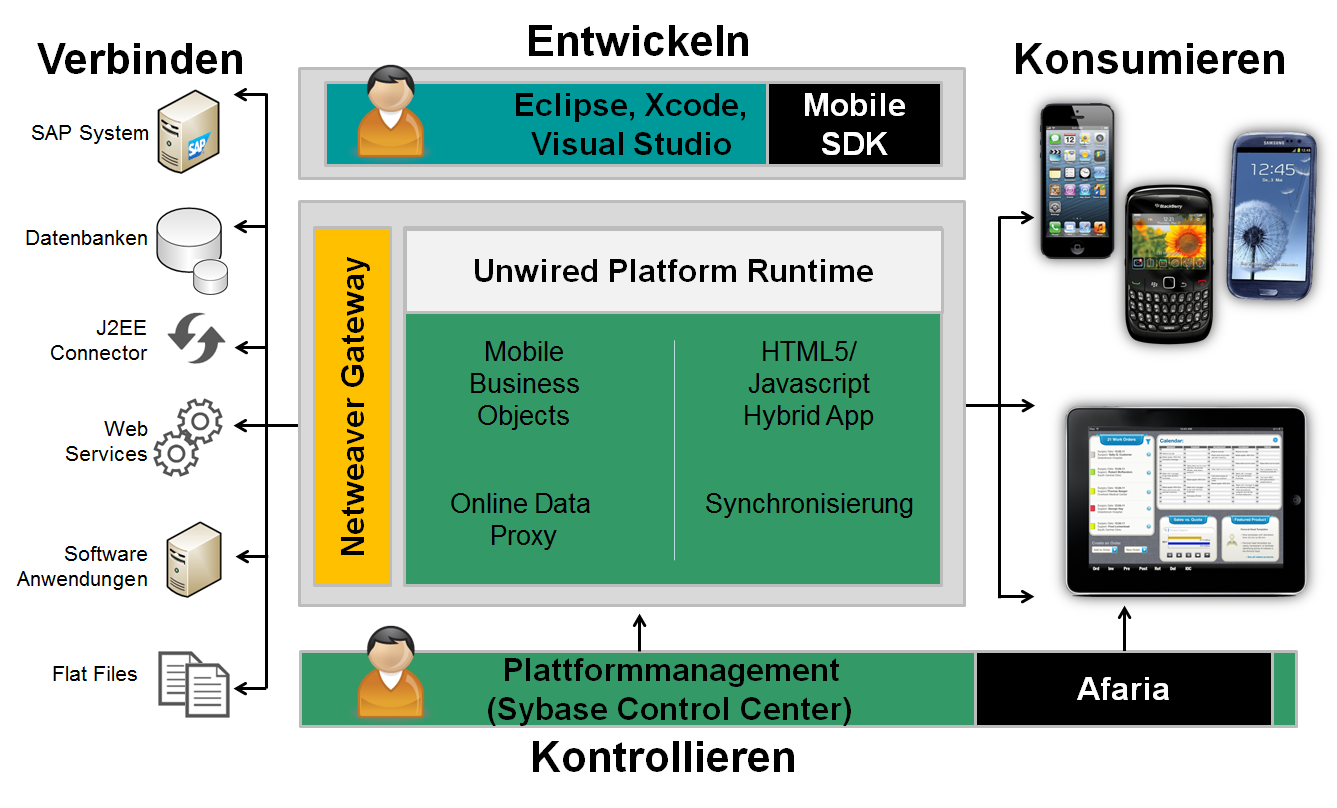
\includegraphics[width=0.9\textwidth]{sup}
\end{lstlisting}

Bei längeren Quellcode-Listings empfiehlt es sich jedoch auf eine externe Datei im Ordner Quellcode zu verlinken und diese einzubauen:
\lstinputlisting[language=HTML]{./Quellcode/Beispiel.html}

Da der Pfad zu den Abbildungen im Hauptdokument definiert wurde, muss hier nur noch der Name des Bildes ohne Dateiendung stehen (sup).


\begin{figure}[H]
\begin{center}
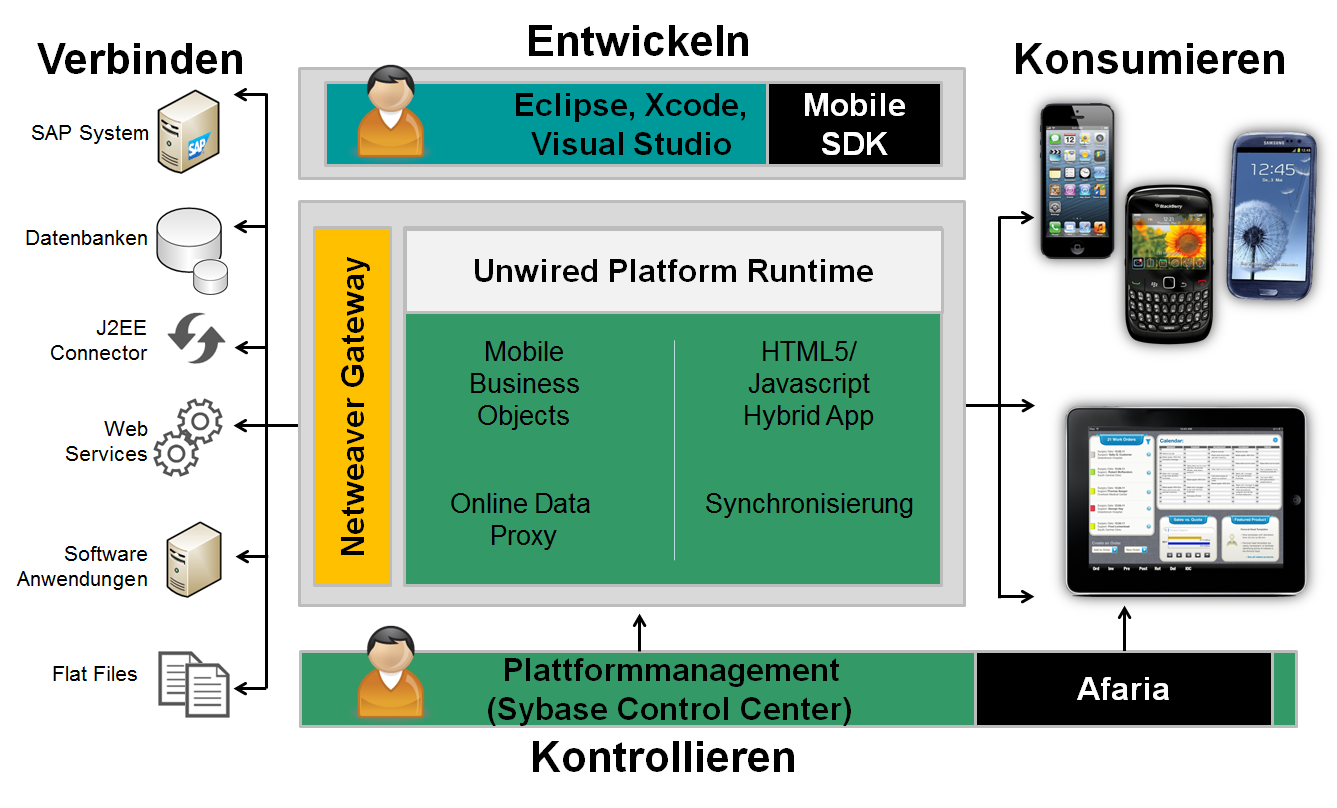
\includegraphics[width=0.9\textwidth]{sup}
\caption{Titel der Abbildung hier}
\end{center}
\end{figure}

\subsection{Tabellen}
\begin{table}[H]
\centering
\begin{tabular}[ht]{|l|l|l|}
  \hline
  \textbf{Abkürzung} & \textbf{Beschreibung} & \textbf{Berechnung}\\
  \hline\hline
    MEK & Materialeinzelkosten & \\
  	MGK & Materialgemeinkosten & $+ \uparrow$~*\\
    FEK & Fertigungseinzelkosten & \\
  	FGK & Fertigungsgemeinkosten & $+ \uparrow$~*\\
	SEKF & Sondereinzelkosten der Fertigung & \\
	\hline\hline
	\multicolumn{3}{|l|}{\textbf{= Herstellungskosten}} \\
	\hline\hline
  	VwGK & Verwaltungsgemeinkosten & $+ \uparrow$~*\\
  	VtGK & Vertriebsgemeinkosten & $+ \uparrow$~*\\
  	SEKVt & Sondereinzelkosten des Vertriebes & \\
	\hline\hline
	\multicolumn{3}{|l|}{\textbf{= Selbstkosten}} \\
	\hline\hline
	\multicolumn{3}{|l|}{+ Gewinnaufschlag} \\
	\multicolumn{3}{|l|}{+ Rabatte} \\
	\hline\hline
	\multicolumn{3}{|l|}{\textbf{= Nettoverkaufspreis (NVP)}} \\
	\hline
	\multicolumn{3}{|l|}{+ Umsatzsteuer} \\
	\hline\hline
	\multicolumn{3}{|l|}{\textbf{= Bruttoverkaufspreis (BVP)}} \\
	\hline
\end{tabular} \\
		\caption{Beispieltabelle 1}
		\label{tbl:beispieltabelle2}
\end{table}

%\clearpage % hiermit werden alle Bilder Tabellen ausgeworfen

\subsection{Biblatex}
Von den vielen verfügbaren Literatur-Paketen habe ich mich für Biblatex entschieden. Die Anforderungen der FOM sollten hiermit erfüllt sein. Ich habe bisher nur Einträge \enquote{@book} getestet. Wie immer steckt der Teufel hier im Detail und es wird sich später herausstellen, ob Biblatex eine gute Wahl war. Die Anpassungen hierfür liegen unter skripte/modsBiblatex. Ich verwende das Backend Biber, welches bib-Dateien in UTF-8 verarbeiten kann.

In der für den Leitfaden 2018 aktualisierten Version sind außerdem Beispiele für \enquote{online},\footcite[Vgl. ][]{website:angular:aboutAngular} also Webseiten, und \enquote{article},\footcite[Vgl. ][S. 140]{Decker2009} also wissenschaftliche Artikel, enthalten.

\subsection{Listen und Aufzählungen}
\subsubsection{Listen}
\begin{itemize}
\item ein wichtiger Punkt
\item noch ein wichtiger Punkt
\item und so weiter
\end{itemize}
\subsubsection{Aufzählungen}
\begin{enumerate}
\item Reihenfolge ist hier wichtig
\item Dieser Punkt kommt nach dem ersten
\item Da sollte jetzt eine 3 vorne stehen
\end{enumerate}

\paragraph{Tiefste Ebene 1}
Dies ist die tiefste Gliederungsebene. Sollten doch mehr Ebenen benötigt werden, muss eine andere Dokumentenklasse verwendet werden.

\paragraph{Tiefste Ebene 2}
Der zweite Punkt in dieser Ebene ist zur Erinnerung daran, dass es nie nie niemals nur einen Unterpunkt geben darf.

\subsection{Skript zum Kompilieren}
Latex will ja bekanntlich in einer bestimmten Reihenfolge aufgerufen werden:
\begin{lstlisting}
pdflatex thesis_main.tex
makeindex thesis_main.nlo -s nomencl.ist -o thesis_main.nls
biber thesis_main
pdflatex thesis_main.tex
pdflatex thesis_main.tex
thesis_main.pdf
\end{lstlisting}

Dies ist der Inhalt der Batchdatei \enquote{compile.bat}.
